% Created 2014-04-14 Mon 15:43
\documentclass[runningheads,a4paper]{llncs}
\usepackage[utf8]{inputenc}
\usepackage[T1]{fontenc}
\usepackage{fixltx2e}
\usepackage{graphicx}
\usepackage{longtable}
\usepackage{float}
\usepackage{wrapfig}
\usepackage{rotating}
\usepackage[normalem]{ulem}
\usepackage{amsmath}
\usepackage{textcomp}
\usepackage{marvosym}
\usepackage{wasysym}
\usepackage{amssymb}
\usepackage{hyperref}
\tolerance=1000
\usepackage[usenames,dvipsnames]{xcolor}
\usepackage[protrusion=true,expansion=true]{microtype}
\usepackage{makeidx}
\usepackage{epstopdf}
\usepackage{times}
\usepackage{listings}
\institute{University of Groningen \and Kings College London \and Brown University}
\hypersetup{plainpages=false}
\setcounter{tocdepth}{3}
\newcommand{\highlight}[1]{\colorbox{yellow}{#1}}
% Autogenerated, do not edit
\newcommand{\revisiondate}{2014-04-24}
<<<<<<< HEAD
\newcommand{\revision}{3f2c73a}
=======
\newcommand{\revision}{d58899a}
>>>>>>> 1b257ee... updates

\author{Kuiper, J\inst{1}. \and Marshall, I.J.\inst{2} \and Wallace, B.C.\inst{3} \and Swertz, M.A.\inst{1}}
\date{\today}
\title{Spá: a web-based viewer for text mining in Evidence Based Medicine}
\hypersetup{
  pdfkeywords={},
  pdfsubject={},
  pdfcreator={Emacs 24.4.50.1 (Org mode 8.2.5h)}}
\begin{document}

\maketitle
\begin{abstract}
When doing sentence extraction or document level predictions on unstructured text the results of trained models are often hard to interpret within their context.
Furthermore presenting results to end users can be a considerable user interface challenge.
These challenges are of key interest in research areas where most findings are only published as unstructured PDF documents, such as evidence based medicine.
To this end we present \textbf{Spá} \footnote{available under GPLv3 at \url{https://github.com/joelkuiper/spa}} \cite{kuiper2014}, a generic web-based visualizer for sentence and document level classifiers on PDFs.
Spá allows the results of sentence extractions to be visualized within the PDF document itself, and allows other results to be presented alongside it.
\\
\\
\texttt{revision: \revision, date: \revisiondate}
\end{abstract}

\section{Introduction}
\label{sec-1}
\begin{figure}[htb]
\centering
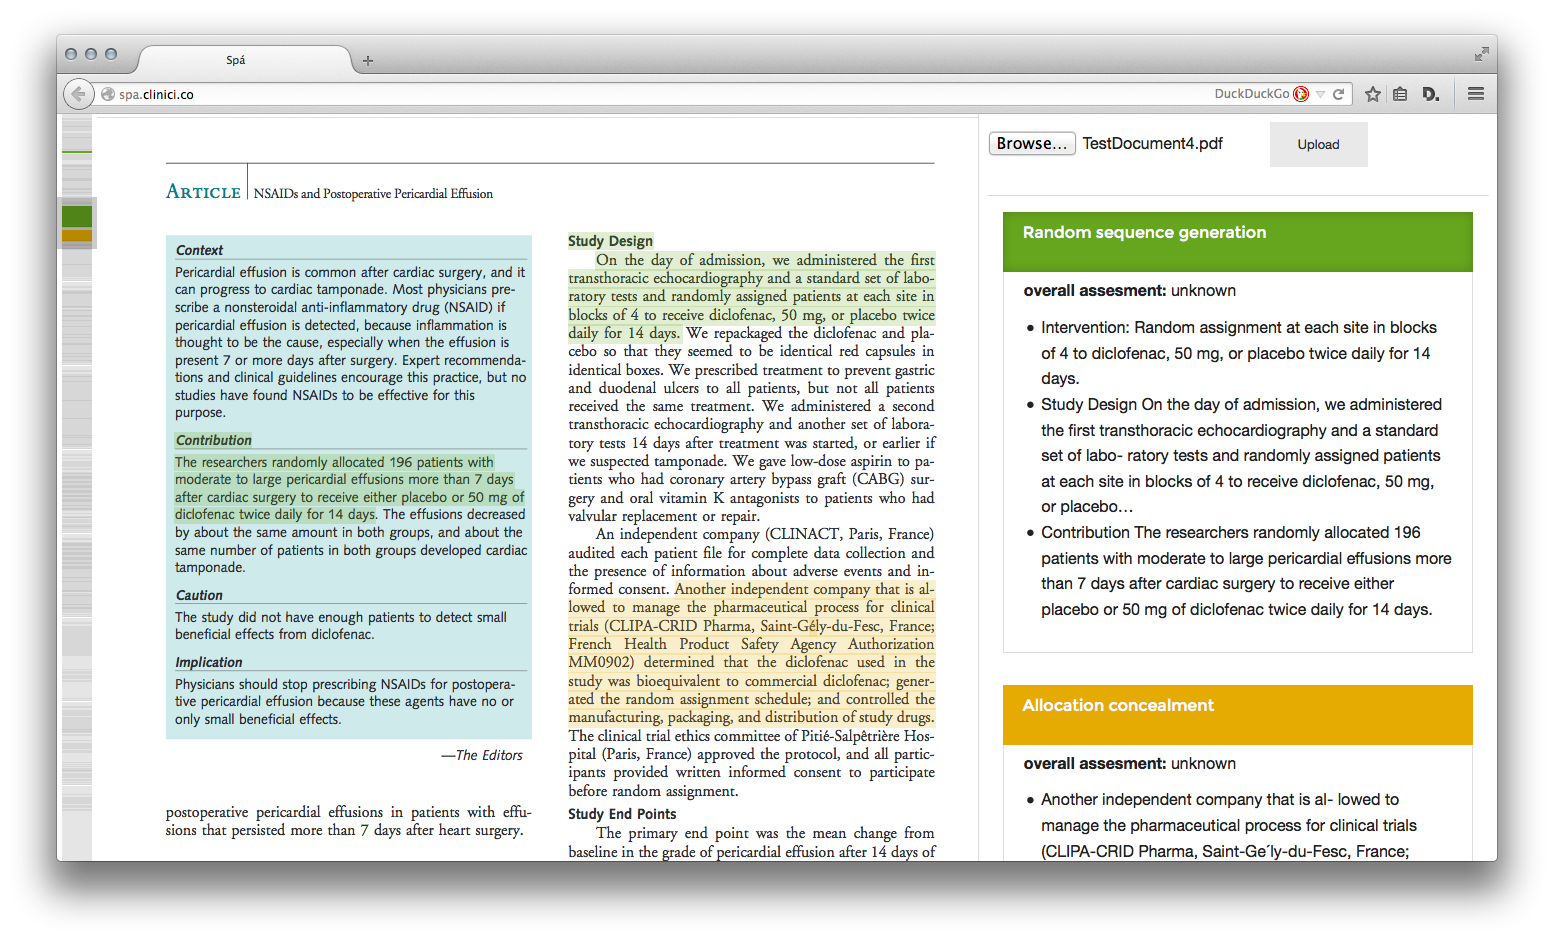
\includegraphics[width=.9\linewidth]{./screenshot.png}
\caption{Screenshot of Spá}
\end{figure}

Finding sentences or words with particular characteristics within a larger document is an important task in natural language processing and machine learning.
For example, one may wish to identify the most important sentences in a document to automatically generate a summary, or match a certain ontology to impose a certain structure.

Dealing with unstructured text is of particular importance in research areas where most findings are only published in that form.
In evidence based medicine, for example, the results of clinical trials, which assess the safety and efficacy of treatments, are often only published as PDF documents.

Furthermore to arrive at informed decisions about a specific clinical question, many clinical trials need to be pooled and summarized.
The process of pooling and summarizing clinical trials is called \emph{systematic reviewing}, and forms the corner-stone of current evidence based medical practice.
Systematic reviewing consists of specifying an inclusion criteria (i.e., the criteria studies must satisfy to be included in the review), searching the literature, screening the retrieved citations to identify eligible studies and, finally, summarizing the relevant evidence.
But achieving this aim is complicated by the massive numbers of trials that are conducted: for example, the Cochrane Library alone indexes 286,418 trials as having been conducted in the last decade \cite{valkenhoef2012}.
While publishing standards are improving and novel tools for systematic reviewing are being created to address this problem \highlight{citation needed}, a lot of legacy publications still only exist as PDF documents.
This raises questions about the sustainability of systematic reviews in its current form.

To aid the process of systematic reviewing we made a generic web-based tool that allows the visualization of annotations within a PDF documents, or meta-information alongside it.
The aim is to have a pluggable system to allow for semi-automated (machine assisted) screening, data extraction and data summarization.
\section{Architecture}
\label{sec-2}

\begin{figure}[htb]
\centering
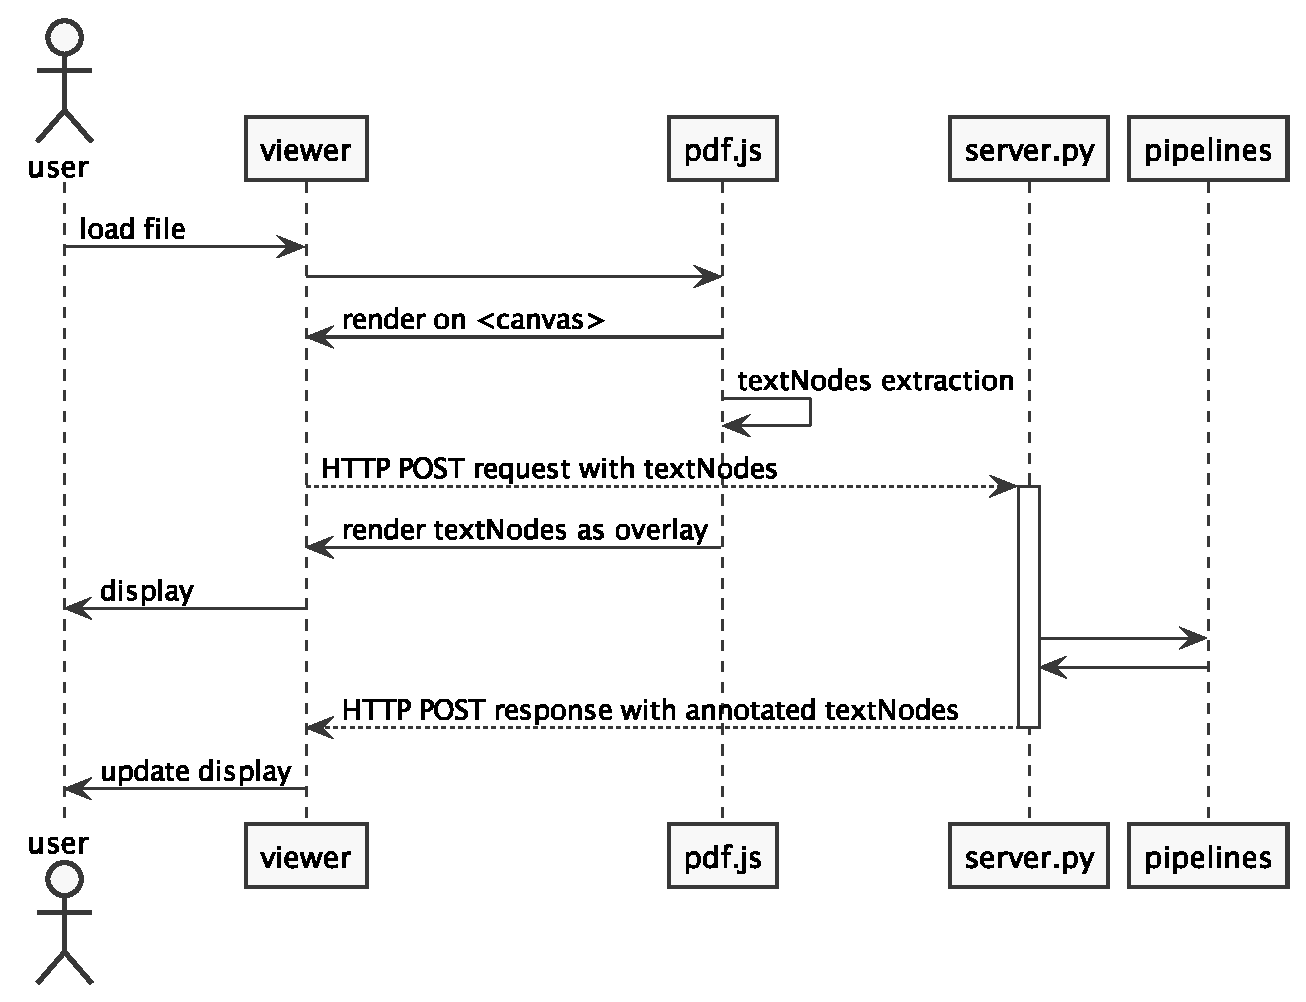
\includegraphics[width=.9\linewidth]{sequence_diagram.eps}
\caption{\label{fig:sequence}Sequence diagram of a typical request-response}
\end{figure}

Spá relies on Mozilla pdf.js\footnote{\url{http://mozilla.github.io/pdf.js}} for visualization of the document and text extraction.
The results of the text extraction are processed server-side by a variety of (pluggable) pipelines, as outlined in figure \ref{fig:sequence}.
Results from these pipelines, which could be complicated machine learning systems, are communicated back to the browser and displayed.
For each of the annotations the relevant nodes in the document are highlighted and a custom scrollbar, inspired by \href{http://substance.io/}{substance.io}, that acts as a mini-map is projected to show where it resides within the document.
The user can then interactively activate and inspect the specific type of results.
\highlight{todo?}
\section{Case Study}
\label{sec-3}
As a case study we evaluate the automatic assessment of Risk of Bias in clinical trial publications.
\highlight{todo}
\section{Conclusion \& Future work}
\label{sec-4}
We present a web-based tool for interactive visualization of annotations and metadata on PDF documents.
This allows users to see the results from machine learning systems within the context of a specific document.
Moreover, we present a case study for Evidence Based Medicine by automatically extracting potential Risks of Bias, with supporting sentences.

However, we believe the tool to be useful for a much wider range of text mining and machine learning applications.
To increase the generality of the tool work is being done to support a consumer/producer protocol for the pipelines, allowing developers to quickly plug in new systems.
Furthermore, work is being done on allowing users to save selected annotations for sharing and off-line, possibly embedded within the document itself.

\bibliographystyle{splncs}
\bibliography{references}
% Emacs 24.4.50.1 (Org mode 8.2.5h)
\end{document}
